\documentclass{beamer}
\usepackage{beamerthemesplit}
\usepackage{wrapfig}
\usetheme{SPbGU}
\usepackage{pdfpages}
\usepackage{amsmath}
\usepackage{cmap} 
\usepackage[T2A]{fontenc} 
\usepackage[utf8]{inputenc}
\usepackage[english,russian]{babel}
\usepackage{indentfirst}
\usepackage{amsmath}
\usepackage{tikz}
\usepackage{multirow}
\usepackage[noend]{algpseudocode}
\usepackage{algorithm}
\usepackage{algorithmicx}
\usepackage{epstopdf}
\usetikzlibrary{shapes,arrows}
\usepackage{fancyvrb}
\newtheorem{rutheorem}{Theorem}
\beamertemplatenavigationsymbolsempty

\title[]{GLL parsing for embedded languages}
\institute[SPbSU]{
Saint Petersburg State University \\
JetBrains Programming Languages and Tools Lab }

\author[Ragozina Anastasiya]{Ragozina Anastasiya}

\date{25/10/2015}

\definecolor{orange}{RGB}{179,36,31}

\begin{document}
{

\begin{frame}
  \begin{center}
  {\includegraphics[width=1cm]{SPbGU_Logo.png}}
  \end{center}
  \titlepage
\end{frame}
}

\begin{frame}[fragile]
  \transwipe[direction=90]
  \frametitle{Problem statement}
  \begin{itemize}
    \item Errors are detected in runtime
    \item IDEs do not provide support (highlighting, brace matching and etc.)
    \item It is necessary to get structure which merges all parse trees --- SPPF
  \end{itemize}
\end{frame}

\begin{frame}
  \transwipe[direction=90]
  \frametitle{Generalised algorithms for embedded languages}  
  \begin{itemize}
    \item Ambiguous grammars are parsed by generalised algorithm (GLL, GLR)
    \item New type of conflict --- ambiguities in the input
    \item Regular approximation of the input is represented as deterministic FSA with tokens on edges
  \end{itemize}
\end{frame}

\begin{frame}
  \transwipe[direction=90]
  \frametitle{GLL for embedded languages}  
  \begin{itemize}
    \item Table-based GLL parsing
    \item Descriptors specify parser state and allow to handle    
  \begin{itemize}
    \item Recursions
    \item Ambiguities
    \item Non-linear input
      \begin{itemize}
        \item Vertex index is used as input position in descriptors
        \item Branching in the input are handled in the same manner as grammar conflicts: the set of descriptors is created
      \end{itemize}
    \item Cycles in input
      \begin{itemize}
        \item Uniqueness of descriptors allows to handle cycles without parsing process changes
      \end{itemize}
    \end{itemize}
    \item  No changes in the process of GSS and SPPF construction
  \end{itemize}
\end{frame}

\begin{frame}
  \transwipe[direction=90]
  \frametitle{Branching in the input}
  \begin{itemize}
    \item For each outgoing edge
    \begin{itemize}
      \item Construct the set of descriptors (as in GLL)
    \end{itemize}
    \item Union all the constructed sets
    \item Example
    \begin{itemize}
      \item Grammar: \texttt{start ::= A C | B C}
      \item Input:
      \item Current vertex index is "0"
      \item Construct two descriptors
      \begin{itemize}
          \item For the edge labeled with "A" \ and grammar rule \texttt{start ::= A C}
          \item For the edge labeled with "B" \ and grammar rule \texttt{start ::= B C}
      \end{itemize}
      \item During parsing process choose the edge which correspond to rule specified in current descriptor 
    \end{itemize} 
  \end{itemize}
\end{frame}

\begin{frame}[fragile]
\transwipe[direction=90]
\frametitle{Static analysis of string-embedded code: the scheme}

\begin{tabular}{p{4.5cm} p{8cm}}
Code: hotspot is marked
&
\begin{minipage}[t]{5cm}

\begin{Verbatim}[commandchars=\\\{\}]
\textcolor{blue}{string} res = \textcolor{orange}{""};
\textcolor{blue}{for}(i = 0; i < l; i++)
    res = \textcolor{orange}{"()"} + res;
\fbox{\textcolor{blue}{use}(res);}

\end{Verbatim}
\end{minipage}

\\ 
Possible values
&
\begin{minipage}[t]{2.5cm}
\begin{Verbatim}[commandchars=\\\{\}]
\{\textcolor{orange}{""}, \textcolor{orange}{"()"},  \textcolor{orange}{"()()"}, ..., \textcolor{orange}{"()"}^l\}
\end{Verbatim}
\end{minipage}

\\
Regular approximation
&
\begin{minipage}[t]{4cm}
  \begin{Verbatim}[commandchars=\\\{\}]
(\textcolor{orange}{"()"})*
  \end{Verbatim} 
\end{minipage}

\\
Approximation
&
\begin{minipage}[t]{3cm}
\raisebox{-\height}{\includegraphics[width=2cm]{pictures/lex1}}
\end{minipage}


\end{tabular}


\end{frame}


\begin{frame}[fragile]
\transwipe[direction=90]
\frametitle{Static analysis of string-embedded code: the scheme}

\begin{tabular}{p{4.5cm} p{8cm}}
\begin{minipage}[t]{4cm}
Approximation\\
\includegraphics[width=2cm]{pictures/lex1}

After lexing\\
\includegraphics[width=3cm]{pictures/in31}

Grammar\\
\vspace{-5pt}
$$
\begin{array}{crcl}
&start &::=& s \\
&s & ::= & \mbox{\texttt{LBR }} s \mbox{\texttt{ RBR }} s\\
&s & ::= &\epsilon
\end{array}
$$
\end{minipage}
&

\begin{minipage}[t]{8cm}
Parse forest\\
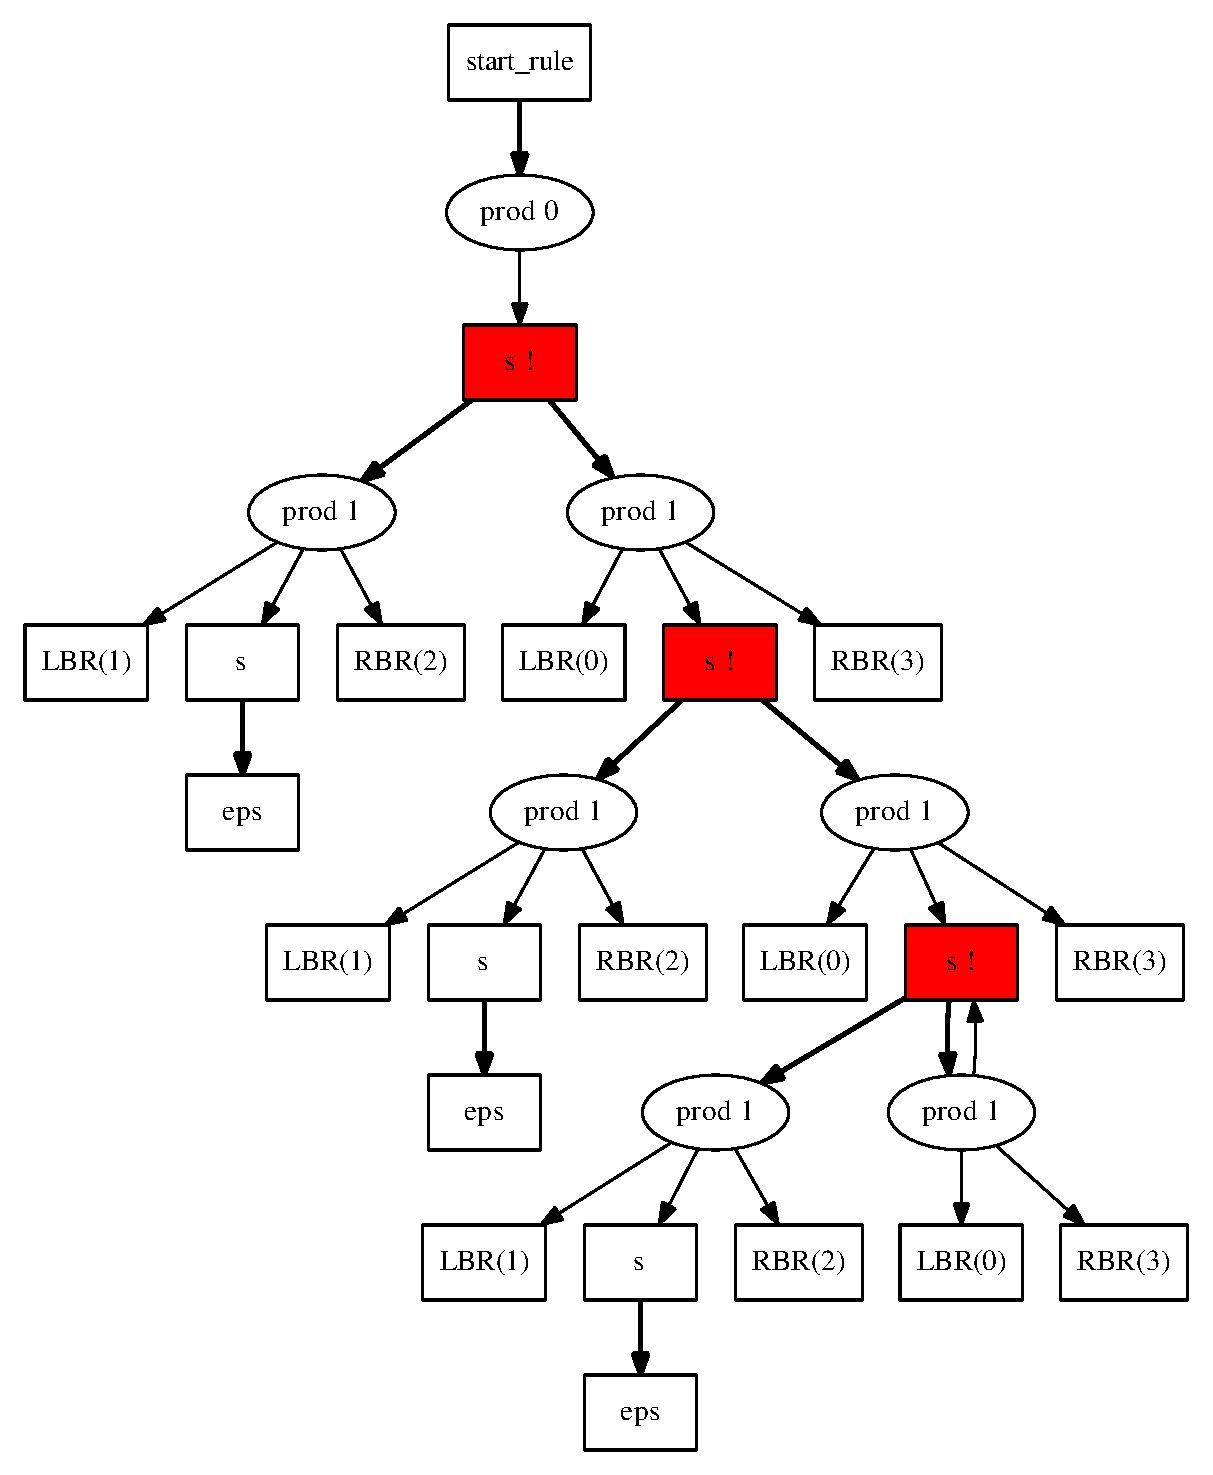
\includegraphics[width=7cm]{pictures/out3}
\end{minipage}

\end{tabular}

\end{frame}


\begin{frame}
  \transwipe[direction=90]
  \frametitle{Conclusion}
  \begin{itemize}
    \item Algorithm based on GLL for parsing of regular approximation of string-embedded code is proposed
    \item Correctness and completeness of the algorithm are proved
    \item The algorithm is implemented and tested in open source project 
    \begin{itemize}
      \item \url{https://github.com/YaccConstructor}
    \end{itemize}

  \end{itemize}
\end{frame}            

\end{document}
